\subsection{Task 3: Model reduction and optimization with improved training efficiency.}

From the effort in \textbf{Task 2}, a robust DNN is available for the practical scenarios. However, DNNs in many scenarios, including medical diagnosis and malware detection, sometimes are deployed on memory-restricted edge devices, such as smartphone and wearable devices. In this task, we aim to compress the developed robust DNN through model pruning technique. 

Model pruning reduces the redundancy in deep neural network for deployment on resource-limited devices. Current model pruning focuses on accuracy guarantee via structural pruning and weight pruning techniques. However, few attention has been paid on the model pruning for robust networks. This project aims at structural pruning on the robust model $\mathcal{M}'$ ({\textbf{Task 2}}) via a generic structural pruning framework. 

Notations and definitions for model pruning are provided firstly.  Let $n$ be the total number of layers, $m_i$ denotes the number of neurons in the layer $l^i$, the robust deep learning model $\mathcal{M}'$ can be presented as $\mathcal{M}'=<L, W, b, \Phi>$, where $L=\{ l^{i}|0\leq i\le n \}$ is a set of layers and $l^0$ denotes the input layer, $W=\{w^i|w^i\in\mathbb{R}^{m_{i-1}\times m_{i}}, 1\le i\le n \}$ is the set of weight matrices, $b=\{b^i|b^i\in\mathbb{R}^{m_i}, 1\le i\le n \}$ is the set of bias vectors, and $\Phi=\{\phi^i|1\le i\le n\}$ is the set of activation functions. Given a model $\mathcal{M}'$, the output vector $o^{i+1}\in\mathbb{R}^{m_{i+1}}$ of layer $l^{i+1}$ ($0\le i\le n-1$) can be defined as:
\begin{equation}
    o^{i+1} = \phi^{i+1}(o^{i}\times w^{i+1} + b^{i+1}).
\end{equation}

% More introductions
Structural pruning aims to remove the redundancy structures in a deep neural network. For layer-wise pruning, the target of structural pruning can be formulized to find a pruning mask $a^i=\{a^{i,j}|a^{i,j}\in\{0,1\}\}^{m_i}_{j=1}$ for layer $l^i$ to satisfy Equation~\eqref{eq:l_pruning}:
 \begin{equation}\label{eq:l_pruning}
 o^{i+1}=\phi^{i+1}(o^i\times w^{i+1}+b^{i+1})\simeq \phi^{i+1}(o^i\circ a^i\times \hat{w}^{i+1}+\hat{b}^{i+1}), 
 \end{equation}
 where $\circ$ denotes the Hadamard product, $\hat{w}^{i+1}$ and $\hat{b}^{i+1}$ denotes new weights and bias to be updated after the pruning. Here, the objective for the pruning is:
 \begin{equation}\label{eq:pruning_target}
     \min(\frac{\beta}{2m_{i+1}}\|o^{i+1} - \phi^{i+1}(o^i\circ a^i\times \hat{w}^{i+1}+\hat{b}^{i+1})\|^2_2),
 \end{equation}
 where $\beta$ denotes the scaling factor.
 
  \begin{figure}[!t]
    \centering
    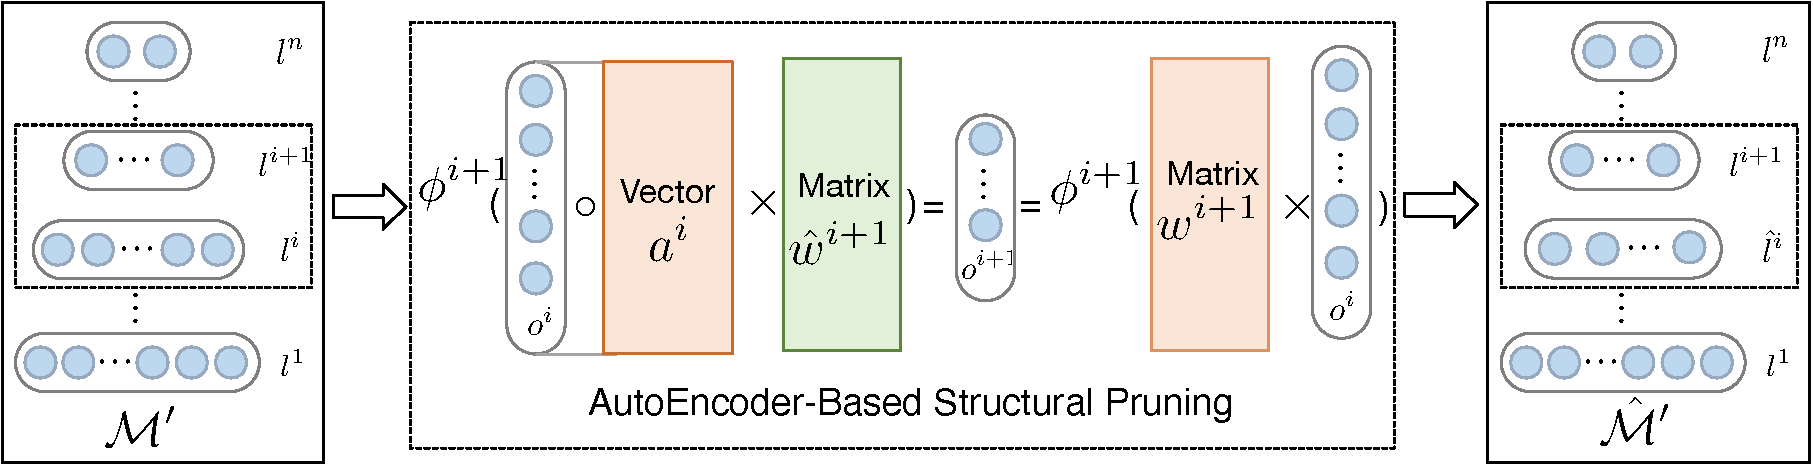
\includegraphics[width=0.9\textwidth]{fig/RP_TASK3_pruning.pdf}
    \caption{Model pruning for robust DNN.}
    \label{fig:task3_pruning}
\end{figure}

 To address the optimization problem in Equation~\eqref{eq:pruning_target}, previous studies~\cite{luo2017thinet, jiang2018efficient} focus on given pruning rates and select the pruning neurons by iteratively updating the binary mask via the greedy selection and weight update. In this project, we propose an auto-encoder-based structural pruning method to learn a binary mask for automatic layer-wise model pruning in Figure~\ref{fig:task3_pruning}. According to Figure~\ref{fig:task3_pruning}, we conduct layer-wise pruning on robust model $\mathcal{M}'$ through the reconstruction of the weight matrix of two adjacent layers. Specifically, motivated by Equation~\eqref{eq:l_pruning}, we use a encoder network to model the mask process and a decoder network to recover the input $o_i$ for layer $l^i$. Here, we iteratively train the binary mask for each layer in model $\mathcal{M}'$ from bottom to top. 
 
 Compared with previous methods, our proposed one enables two advantages: (1) Our method selects the pruning neurons automatically without a specified pruning rate; (2) The by-product of the structure $\hat{w}^{i+1}$ for layer $l^i$ is performance-preserving and no extra fine-tuning process is required. Here, considering the input $a^i$ of this auto-encoder is data-related ($a^0$ in the first layer is actually the input data), the parameters in this autoencoder can be updated by the training set. Regrading the optimization-enabled update process, the objective function is composed of the following parts:
\begin{itemize}
    \item Reconstruction loss. Reconstruction loss aims to guarantee the minimum distance of the outputs of the encoder and decoder. The Reconstruction loss can be presented as:
    \begin{equation}\label{eq:reconstruction_loss}
        \mathcal{L}_{RC} =  
     \frac{\alpha}{2m_{i+1}}\|\phi^{i+1}(o^i\times w^{i+1}+b^{i+1}) - \phi^{i+1}(o^i\circ a^i\times \hat{w}^{i+1}+\hat{b}^{i+1})\|^2_2,
    \end{equation}
    where $\alpha$ denotes the scaling factor.
    \item Maximum pruning loss. Maximum pruning loss aims to remove the weights in a layer to the utmost extent. considering the pruning mask is a binary vector, the maximum pruning loss can be presented as:
    \begin{equation}
        \mathcal{L}_{MP} = \beta \sum_{j=1}^{m_{i+1}} a^{i,j},
    \end{equation}
    where $\beta$ denotes the balancing coefficient.
    \item Performance-preserving loss. To maintain the robustness of the robust $\mathcal{M}'$, the trained encode vector is expected to be close with the initial encoder vector $o^{i+1}$, the loss can be presented as:
    \begin{equation}
        \mathcal{L}_{PP} =  \frac{\gamma}{2m_{i+1}}\|o^{i+1} - \phi^{i+1}(o^i\circ a^i\times \hat{w}^{i+1}+\hat{b}^{i+1})\|^2_2,
    \end{equation}
    where $\gamma$ denotes the scaling factor.
\end{itemize}

Finally, the loss for the optimization $\mathcal{L}_{pruning}$ is:
\begin{equation}
    \mathcal{L}_{pruning} = \mathcal{L}_{RC}+\mathcal{L}_{MP}+\mathcal{L}_{PP}.
\end{equation}

Noted that original binary network is hard to converge, here soft mask technique is utilized ($a^i=\{a^{i,j}|a^{i,j}\in \mathcal{R}^{m_i}_{j=1}, 0\le a^{i,j}\le 1$). In addition, two-step optimization from FISTA~\cite{denton2014exploiting} is introduced to solve the optimization of $a^i$ and $\hat{w}^i$.

After the iteration of the structural pruning, we can obtain a pruned model $\mathcal{M}^{''}$, where the new structure in layer $l^i$ and the corresponding weights $\hat{w}^{'}$ are from the trained auto-encoder. In this project, we will further explore the formal verification techniques in \textbf{Task 4} to verify the preserved robustness of the pruned model $\mathcal{M}^{''}$ and certificate it with a quantified score.